\documentclass[a4paper,10pt]{article}
\usepackage[utf8]{inputenc}
\usepackage[spanish]{babel}
\usepackage[pdftex]{graphicx}

\makeindex

%opening
\title{\underline{\textbf{Filesystems, IPCs y Servidores Concurrentes}}}
\author{
Lezica, Santiago. (Leg. 49147).\\
Ballesty, Pablo Andrés. (Leg. 49359).\\
Pose, Jimena Belén. (Leg. 49015).\\
}
\date{}

\begin{document}

\maketitle

\newpage
\tableofcontents

\newpage
\section{Introducción}
\subsection{Objetivo}
El objetivo de este trabajo es familiarizarse con el uso de sistemas cliente-
servidor concurrentes, implementando el servidor mediante la creación de proce-
sos hijos utilizando fork() y mediante la creación de threads. Al mismo tiempo,
ejercitar el uso de los distintos tipos de primitivas de sincronización y comunicación
de procesos (IPC) y manejar con autoridad el filesystem de Linux desde
el lado usuario.

\subsection{Enunciado}
Se desea implementar un simulador de colonia de hormigas simplificado. En
el mismo habrá un hormiguero, varias hormigas y comida esparcida a lo largo
del mundo. Las hormigas deberán recolectar la comida y traerla al hormiguero.
Para ello deberán leer la información del ambiente y comunicarse entre ellas
de manera eficiente. El objetivo de la simulación es traer la mayor cantidad
de comida al hormiguero. Después de 10000 turnos, o cuando ya no haya más
comida en el mundo, la simulación finaliza.\\
El servidor leerá del archivo de configuración la información acerca del mundo,
que tendrá forma de grilla. Particularmente estará la ubicación del hormiguero,
cada pieza de comida, su tipo (simple o grande) y las hormigas en su posición inicial.
A continuación, empezará la simulación, en donde, por turnos simultáneos, to-
das las hormigas deberán realizar una acción. Esta acción podría ser o bien:

\begin{enumerate}
 \item Moverse a un casillero contiguo horizontal o vertical.
 \item Oler los casilleros vecinos para detectar rastros, hormigas o comida.
 \item Levantar una pieza de comida que esté en un casillero contiguo horizontal o vertical.
 \item Moverse a un casillero vecino dejando un rastro.
 \item Emitir un grito.
\end{enumerate}

Dos hormigas no podrán ocupar el mismo casillero y 1 hormiga no podrá ocupar 
el mismo casillero que una pieza de comida sin levantar. En caso de que al
finalizar un turno, 2 o más hormigas intenten moverse al mismo casillero, solo
una lo logrará y la otra fallará su movimiento. La unica excepción a esta regla
es el hormiguero. Pueden haber infinitas hormigas en el casillero del hormiguero.
Las hormigas pueden dejar y detectar un rastro. Este rastro es un valor decimal
entre 0 y 1, en donde 1 es un rastro recién puesto y 0 es ”no hay rastro en
absoluto”. Al avanzar y dejar rastro, el valor de rastro dejado SIEMPRE será 
de valor 1. y por cada turno el rastro decrementará en 0.01.\\

Las hormigas SIEMPRE saben la orientación del hormiguero relativa a donde
están paradas, no así la distancia. (Es decir, una hormiga puede preguntar, sin
invertir turnos en ello, hacia donde está el hormiguero y recibir como respuesta
(N,S,E,W,NE,NW,SE,SW).\\

Las hormigas tienen una memoria muy limitada y solo pueden recordar 2 posiciones 
en el mapa, una de ellas siendo siempre el hormiguero. Es decir, una
hormiga puede decidir almacenar una posición del tablero para luego preguntarse
en que dirección está.\\

Las hormigas tienen una memoria muy limitada y solo pueden recordar 2 posiciones 
en el mapa, una de ellas siendo siempre el hormiguero. Es decir, una
hormiga puede decidir almacenar una posición del tablero para luego preguntarse
en que dirección está.
Cuando una hormiga grita, todas las hormigas reciben la posición de la hormiga
que grita y la distancia hamiltoniana entre ellas. Al escuchar un grito, una
hormiga puede optar por reemplazar su memoria por la posición de la hormiga
que gritó.\\

Existen 2 tipos de comida: chica y grande. La comida chica puede ser transportada 
por una hormiga sin dificultad y tiene valor 1. La hormiga simplemente
tiene que posicionarse en un casillero contiguo y utilizar un turno para levantar
la comida. La comida grande vale 5 puntos, puede ser transportada por una
hormiga, pero necesita de 2 hormigas para ser levantada, es decir: debe haber
2 hormigas posicionadas contigua a la comida y ambas deben utilizar un turno
para levantar o asistir en levantar la comida.\\

\subsection{Actividades}
Implemente la simulación utilizando procesos y threads y haga cuatro versiones del sistema, 
usando las siguientes primitivas de IPC:
\begin{enumerate}
 \item 
    \begin{itemize}
      \item Pipes o fifos.
      \item Colas de mensajes - System V o POSIX.
      \item Memoria compartida o mmap(), Semáforos System V o POSIX.
      \item Sockets - TCP o de dominio Unix.
    \end{itemize}
  \item El archivo de configuración tendrá el siguiente formato:
    \begin{itemize}
     \item Una línea con la longitud y alto del tablero separados por coma. Ej: 6,8
      significa un tablero de 6 columnas y 8 filas.
     \item Una línea con la posición del hormiguero separada por coma, teniendo en
      cuenta que la posición superior izquierda es 0,0. Ej: 3,4 significa que el
      hormiguero está en la cuarta columna, quinta fila.
     \item Una línea con la cantidad de hormigas N. Todas las hormigas empiezan
      en el hormiguero.
     \item Una línea con la cantidad de comida chica M, seguida de M líneas con la
      posición de cada comida.
     \item Una línea con la cantidad de comida grande K, seguida de K líneas con la
      posición de cada comida.
    \end{itemize}
  \item El programa debe permitir la visualización de la simulación en un tablero en
   la pantalla, iterando turno a turno.
  \item Todas las hormigas deben tener la misma programación, es decir, si bien
  lo que hacen dependerá de su posición y pueden elegir moverse a un lugar al
  azar, debe haber una unica función con la programación para todas las hormigas
  individuales.
  \item La nota del trabajo prático no dependerá de la eficiencia de la simulación,
   sin embargo, la cátedra proveerá 3 escenarios de prueba y se otorgará un punto
    extra al equipo que maximice puntajes en estos 3 escenarios.

\end{enumerate}

\newpage

\section{Desarrollo}
\subsection{Modelado del problema}
Para el desarrollo de la simulación de hormigas decidimos modelar a cada hormiga como un proceso, el cual dispara un \textit{thread} que se
encarga de la comunicación de esta hormiga con el \textit{server}. De la misma manera, el \textit{server} es un proceso que dispara un thread
que se encarga de la comunicación de éste con las hormigas de este mini-universo.\\
Los \textit{threads} aprovechando que comparten los datos con el proceso que los dispara, se encargarán de recibir y enviar constantemente los 
mensajes entrantes y salientes, a través de los distintos sistemas de \textbf{IPC}, estos mensajes entrantes y salientes serán debidamente
encolados o desencolados de las colas \textit{inbox} y \textit{outbox} que posee cada proceso en ejecución.\\
A continución se coloca una ilustración de un server conectado con dos hormigas:

\begin{center}
 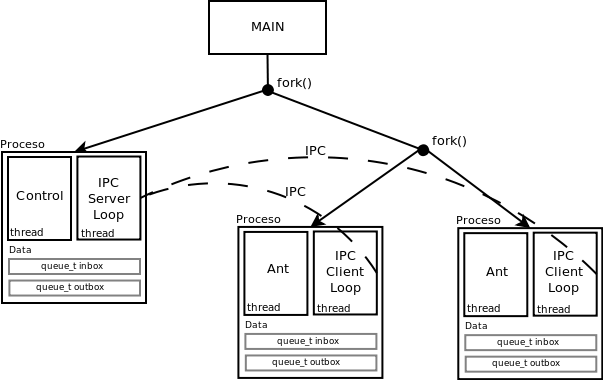
\includegraphics[scale=0.65]{./so1.png}
 % so1.png: 603x380 pixel, 72dpi, 21.27x13.41 cm, bb=0 0 603 380
\end{center}

\newpage
\subsection{Implementación de IPCs}
\subsubsection{Fifos}
Para entablar una comunicación entre procesos mediante el sistema de IPC implementado con \textbf{FIFOS}, se tomaron las siguientes decisiones:
\begin{itemize}
 \item Al iniciar el proceso, el \textit{server} creará en el directorio ``/tmp'', todas las fifos necesarias para entablar comunicación 
con las \textit{n} hormigas participantes.
 \item Los nombres de cada fifo corresponden a la siguiente regla: La hormiga con id lógico \textit{n} enviará mensajes a través de la fifo 
``\verb|/tmp/fifo_c_w_n|'' y recibirá mensajes a través de la fifo ``\verb|/tmp/fifo_c_r_n|''. De esta manera entabla una comunicación
bidireccional con el \textit{server}.
  \item Se asume que en el directorio ``/tmp'' no hay fifos creadas con los mismos nombres, el programa se asegura crear y eliminar todas las 
fifos utilizadas.
\end{itemize}


\subsubsection{Colas de mensajes}
Para la versión del sistema que utiliza \textbf{Colas de mensajes} se decidió utilizar \textbf{System V} para poder tener una única cola y 
manejar los mensajes con prioridades. De esta manera se mantiene siempre una prioridad para cada proceso, siendo esta su sid (simulation id).
En el caso del servidor, el sid siempre es 1 (Debido a que si se intentan levantar mensajes con prioridad 0 de la cola, esta devuelve el de menor 
prioridad, es decir que se toma como prioridad por defecto), y para las hormigas es n + 1.\\
Cuando se inicia el servidor se dispara un thread que entra en un loop infinito levantando mensajes con la prioridad del servidor e 
insertándolos en la cola con el número de prioridad a quien está dirigido el mensaje (indicado en la estructura st\_msg\_t), a no ser que esté 
dirigido a él, en ese caso lo inserta en la \textit{inbox} del servidor.\\
Por otro lado, al iniciarse cada cliente se dispara un nuevo thread, que también entra en un loop infinito, levanta mensajes de la cola 
con la prioridad del cliente y los inserta en su \textit{inbox}. Este mismo thread a la vez agarra los mensajes de la \textit{outbox} del 
cliente y los inserta en la cola de mensajes con la prioridad del servidor.\\
Por último, si se intenta levantar un mensaje de la cola con una prioridad determinada y la cola no tiene ningún mensaje con esta prioridad se 
decidió que el proceso no se bloquee hasta encontrar dicho mensaje, si no que siga pidiendo mensajes hasta que haya uno, para que el resto de los 
procesos puedan seguir enviando y recibiendo mensajes normalmente.\\
Gracias a la propuesta de \textbf{System V} se logró utilizar una única cola de mensajes para comunicar varios procesos.

\subsubsection{Memoria compartida y semáforos}
Para la implementación del IPC con \textbf{Memoria compartida} se utilizó la propuesta de \textbf{System V} para allocar memoria compartida, y 
2 semáforos binarios o locks.
Se crearon dos buffers circulares, en uno el proceso \textit{server} escribe los mensajes para los clientes y en el otro lee los mensajes que
le envían. En cada acceso a cada buffer, se utiliza un lock para evitar problemas de sincronización.\\
A su vez cada cliente, lee del buffer donde el server escribe, y escribe en el buffer de donde lee el server, siempre lockeando en los accesos.
De esta manera se logra una comunicación bidireccional entre un proceso cliente y un proceso server.

\subsubsection{Sockets}

La implementación del sistema con sockets utiliza el modelo de comunicación orientado a conexiones, estableciendo la comunicación entre todos los procesos hormiga y el servidor-control de simulación. Se utilizaron sockets de la familia de direcciones INET, bajo protocolo TCP.

Al iniciarse el thread de comunicación en el servidor, un socket no-bloqueante escucha en una dirección pública, conocida por todos los procesos del programa, y dispara un nuevo thread cada vez que llega una solicitud de conexión.

Los threads controlan el envío y la recepción de datos de cada cliente, vaciando una outbox propia y populando una inbox, también propia (ambas colas thread-safe, multi-producer y multi-consumer). El thread principal de comunicaciones, a su vez, traslada los mensajes entrantes de las inbox de cada cliente a una cola general de mensajes de entrada que el thread de control de simulación puede acceder. En el sentido inverso, cuando el control decide enviar un mensaje, lo encola en una bandeja de salida general y el thread de servicio se encarga de llevar el mensaje a la bandeja de salida individual del cliente correspondiente.

En todo momento se utilizan sockets no bloqueantes, iterando sobre una máquina de estados que recibe los headers y datos de los mensajes, en forma busy. Entendemos que la baja performance que resultó tener esta implementación tiene su origen en esta decisión de diseño cuestionable: ninguno de los múltiples threads y procesos del programa bloquea o duerme, de manera que el cambio constante de contexto y el acceso permanente a objetos protegidos por exlcusión mutua reducen el ritmo de ejecución de forma muy notoria.

\newpage
\subsection{Desarrollo y decisiones de la lógica de simulación}

\subsubsection{Desarrollo de entrada y salida}
Para mostrar la simulación en pantalla se decidió usar ncurses gracias a la recomendación de la cátedra, lo que facilitó la visualizacion de los 
datos. Debido a que la terminal con la cual se cuenta solo ofrece 8 colores predefinidos se decidió crear una escala lo más apropiada posible 
para mostrar los rastros de las hormigas en color en la pantalla. Por este mismo motivo se puede ver una referencia con los valores de la escala 
en la parte inferior de la pantalla. En esta referencia también se puede ver el significado de los símbolos que aparecen en el tablero.\\
En cuanto al archivo de configuración, llamado \textit{configurationFile}, se toma en cuenta que está bien formado, es decir que los datos 
aparecen tal cual como están descriptos en el enunciado. Se asume que no hay líneas en blanco entre una línea de información y otra, y que no 
hay espacios en blanco al final de cada línea.


\subsubsection{Lógica del Servidor}
El servidor será el encargado de responder a los comandos enviados por las hormigas, para ello, posee un arreglo de punteros a función, el cuál utiliza
el tipo de comando recibido como índice de ese arreglo, localizando la función \textit{handler} de ese comando en \textbf{$O(1)$}; esta característica es
una gran ventaja, ya que hace a la lógica totalmente escalable, y asegura su futura eficiencia.
Para la simulación de las hormigas, el server recibe los siguientes tipos de comandos:
\begin{itemize}
 \item CMD\_START
 \item CMD\_MOVE\_REQ
 \item CMD\_SMELL\_REQ
 \item CMD\_PICK\_REQ
 \item CMD\_YELL\_REQ
 \item CMD\_STOP
\end{itemize}
Cuando la lógica de server comienza, espera que todas las hormigas le envíen CMD\_START, y de esta manera se van marcando en estado ANT\_READY 
en un arreglo de hormigas.
Cuando todas se encuentran en ANT\_READY, comienza la simulación propiamente dicha, envíando el server el comando CMD\_TURN a todas las hormigas,
estas contestarán con CMD\_MOVE\_REQ, CMD\_SMELL\_REQ, CMD\_PICK\_REQ ó CMD\_YELL\_REQ, y cada una pasará por su correspondiente función 
\textit{handler} las cuales modificarán el estado de la hormiga a ANT\_DECIDED, si el turno no require de ningún procesamiento más, y sino, como en el
caso de CMD\_MOVE\_REQ o CMD\_PICK\_REQ utilizarán estados intermedios, para luego de haber procesado todas las decisiones, resolver los problemas
de concurrencia, y dejar a la hormiga en el estado ANT\_DECIDED.\\
Cuando todas las hormigas se encuentren en el estado ANT\_DECIDED, el server pasará a enviar los comandos de respuesta a cada hormiga, los cuales
ya se encuentran alojados en el arreglo de información que guarda internamente.\\
En el caso de CMD\_YELL\_REQ, enviará la respuesta CMD\_YELL\_RES a la hormiga que envío el comando, y dejará marcado en el arreglo de información, que
se les debe avisar a las demás hormigas de los sucedido, esto lo hace luego de enviar las respuestas a las hormigas, enviando CMD\_YELL\_NOT.\\
Esta lógica se repetirá hasta cumplirse los 10000 turnos, o haberse acabado la comida del mundo. Cuando esto suceda, el server enviará a las hormigas
CMD\_STOP, y esperará hasta que estas le respondan con el mismo mensaje, marcando esto en el arreglo de información, cuando todas hayan respondido,
se detiene al thread de comunicación, y se destruyen la memoria y demás partes utilizadas para los IPCs, para luego terminar con la simulación.

\newpage
\section{Conclusiones}
Al finalizar el Trabajo Especial, concluímos en que, nuestra API de IPCs brindaba ventajas que la simulación pedida no requería, por ejemplo, el envío
de mensajes de tamaño variable y la lógica de comunicación no bloqueante. Trabajo que nos demoró mas tiempo de lo esperado, pero que no consideramos
en vano, ya que nos enfrentó a nuevos desafíos que logramos superar; por este motivo se nos retrasó el desarrollo de la lógica de simulación, por lo que
no logramos desarrollar una hormigas muy inteligentes. Sin embargo, creemos haber ganado más de lo perdido.

\bigskip
\end{document}
